\documentclass[3pt,landscape]{article}
%ss[10pt,landscape]{article}
\usepackage{multicol}
\usepackage{calc}
\usepackage{ifthen}
\usepackage[landscape]{geometry}
\usepackage{amsmath,amsthm,amsfonts,amssymb}
\usepackage{color,graphicx,overpic}
\usepackage{hyperref}


\pdfinfo{
/Title (final.pdf)
/Creator (TeX)
/Producer (pdfTeX 1.40.0)
/Author (Raemond Bergstrom-Wood)
/Subject (Algorithms)
/Keywords (pdflatex, latex,pdftex,tex)}

% This sets page margins to .5 inch if using letter paper, and to 1cm
% if using A4 paper. (This probably isn't strictly necessary.)
% If using another size paper, use default 1cm margins.
\ifthenelse{\lengthtest { \paperwidth = 11in}}
    { \geometry{top=.3in,left=.3in,right=.3in,bottom=.3in} }
    {\ifthenelse{ \lengthtest{ \paperwidth = 297mm}}
        {\geometry{top=1cm,left=1cm,right=1cm,bottom=1cm} }
        {\geometry{top=1cm,left=1cm,right=1cm,bottom=1cm} }
    }

% Turn off header and footer
\pagestyle{empty}

% Redefine section commands to use less space
\makeatletter
\renewcommand{\section}{\@startsection{section}{1}{0mm}%
                            {-1ex plus -.5ex minus -.2ex}%
                            {0.5ex plus .2ex}%x
                            {\normalfont\large\bfseries}}
\renewcommand{\subsection}{\@startsection{subsection}{2}{0mm}%
                            {-1explus -.5ex minus -.2ex}%
                            {0.5ex plus .2ex}%
                            {\normalfont\normalsize\bfseries}}
\renewcommand{\subsubsection}{\@startsection{subsubsection}{3}{0mm}%
                            {-1ex plus -.5ex minus -.2ex}%
                            {1ex plus .2ex}%
                            {\normalfont\small\bfseries}}
\makeatother

% Define BibTeX command
\def\BibTeX{{\rm B\kern-.05em{\sc i\kern-.025em b}\kern-.08em
    T\kern-.1667em\lower.7ex\hbox{E}\kern-.125emX}}

% Don't print section numbers
\setcounter{secnumdepth}{0}


\setlength{\parindent}{0pt}
\setlength{\parskip}{0pt plus 0.5ex}

%My Environments
\newtheorem{example}[section]{Example}
% -----------------------------------------------------------------------

\def\ci{\perp\!\!\!\perp}

\begin{document}
\raggedright
\footnotesize
\begin{multicols}{3}


% multicol parameters
% These lengths are set only within the two main columns
%\setlength{\columnseprule}{0.25pt}
\setlength{\premulticols}{1pt}
\setlength{\postmulticols}{1pt}
\setlength{\multicolsep}{1pt}
\setlength{\columnsep}{2pt}

\begin{center}
    \Large{\underline{CS 170 Final Cheat Sheet}} \\
\end{center}

\subsection*{Formal Limit Definition of \(O, \Theta, \texttt{and } \Omega\)}
\[\lim_{n \rightarrow \infty}\frac{f(n)}{g(n)}\left\{\begin{array}{lr}
            \geq 0(\infty) & f(n) \in \Omega(g(n))\\
            < \infty(0) & f(n) \in O(g(n))\\
            = c, 0 < c < \infty & f(n) \in \Theta(g(n))
    \end{array}\right.\]

\subsection*{Euclid's GCD: \(O(n^{3})\)}
\begin{verbatim}
def gcd(a,b):
    if b==0:
        return a
    return gcd(b, a mod b)
\end{verbatim}

\subsection*{Extended GCD: \(O(n^{3})\)}
\begin{verbatim}
def extended-gcd(a,b):
    if b==0:
        return (1, 0, a)
    (x', y', d) = extended-gcd(b, a mod b)
    return (y', x' - floor(a/b)*y', d)
\end{verbatim}
if d divides a and b and \(d=ax+by\) for some integers s and y,\\
then d = gcd(a, b)

\subsection*{Multiplicative Inverse}
inverse of a,
\[ax \equiv 1 (\texttt{mod } N)\]
for any \(a (\texttt{mod } N)\), a has a multiplicative inverse if and only if they are relatively prime, gcd(a,N) = 1

\subsection*{Fermat's Little Theorem}
given a prime (or carmichael) p,
\[a^{p-1} \equiv 1 (\texttt{mod } p)\]
Proof:\\
Given a set of numbers, \(S = \{1,2,\ldots,p-1\}\) modulo p, there is a 1 to 1 mapping of numbers in S to thier inverses also in S\\
Then we can also say, \[S = \{a*1(\texttt{mod }p), a*2(\texttt{mod }p), \ldots, a*(p-1)(\texttt{mod }p)\}\]
Multiplying all of these numbers together gives us,
\[(p-1)! \equiv a^{p-1}\cdot(p-1)!(\texttt{mod }p)\]
Here we can divide by \((p-1)\)! (which we can do because it is relatively prime to p)
\[a^{p-1} \equiv 1(\texttt{mod }p)\]

\subsection*{RSA Euler's Theorem}
\[m^{(p-1)(q-1)}=1 (\texttt{mod } p)\]

\subsection*{Master's Theorem}
If
\[T(n)=aT(\lceil n/b \rceil)+O(n^{d}) \texttt{ for } a>0,b>1 \texttt{, and } d\geq 0,\]
then,
\[T(n)=\left\{\begin{array}{lr}
            O(n^{d}) & if d>log_{b}a\\
            O(n^{d}logn) & if d=log_{b}a\\
            O(n^{log_{b}a}) & if d < lob_{b}a
        \end{array}
        \right.\]

\subsection*{Volker Strassen}
Divide and conquer matrix multiplication.\\
Matrix multiplication can be broken into subproblems, because it can be performed blockwise. Ex, we can carve X into for \(n/2\) x \(n/2\) blocks
\[X = \begin{bmatrix} A & B \\ C & D \end{bmatrix}, Y = \begin{bmatrix} E & F\\ G & H \end{bmatrix}\]
Then the product can be expressed in terms of those blocks as if the blocks were a single element,
\[XY = \begin{bmatrix} A & B \\ C & D \end{bmatrix} * \begin{bmatrix} E & F\\ G & H \end{bmatrix} = \begin{bmatrix} AE+BG & AF+BH \\ CE+DG & CF+DH \end{bmatrix}\]
The runtime of this recurrence is,
\[T(n)=8T(n/2)+O(n^{2}) \rightarrow O(n^{3})\]
Using clever algebra, this can be improved with integer multiplication, XY can be computed from seven \(n/2\) x \(n/2\) subproblems via decomposition.
\[XY = \begin{bmatrix} P_{5}+P_{4}-P_{2}+P_{6} & P_{1}+P_{2} \\ P_{3}+P_{4} & P_{1}+P_{5}-P_{3}+P_{7} \end{bmatrix}\]
where,
\[\begin{array}{ll}
        P_{1}=A(F-H) & P_{2}=(A+B)H\\
        P_{3}=(C+D)E & P_{4}=D(G-E)\\
        P_{5}=(A+D)(E+H) & P_{6}(B-D)(G+H)\\
        P_{7}=(A-C)(E+F) & \texttt{ }
\end{array}\]
and has a runtime of
\[T(n)=7T(n/2)+O(n^{2}) \rightarrow O(n^{log_{2}7}) \approx O(n^{2})\]

\subsection*{Fast Fourier Transform}
complex \(n^{th}\) roots of unity are given by \(e^{\frac{2 \pi i}{n}}\)
The Vandermonde Matrix,
\[M_{n}(\omega) =
    \begin{bmatrix}
        1 & 1 & 1 & \cdots & 1\\
        1 & \omega & \omega^{2} & \cdots & \omega^{n-1}\\
        1 & \omega^{2} & \omega^{4} & \cdots & \omega^{2(n-1)}\\
        \vdots & \vdots & \vdots & \ddots & \vdots\\
        1 & \omega^{j} & \omega^{2j} & \cdots & \omega^{(n-1)j}\\
        \vdots & \vdots & \vdots & \ddots & \vdots\\
        1 & \omega^{(n-1)} & \omega^{2(n-1)} & \cdots & \omega^{(n-1)(n-1)}
\end{bmatrix}\]

\subsection*{Search Algorithms}
\subsubsection*{Depth First Search}
\begin{verbatim}
def explore(G,v): #Where G = (V,E) of a Graph
    visited(v) = true
    previsit(v)
    for each edge(v,u) in E:
        if not visited(u):
            explore(u)
    postvisit(v)

def dfs(G):
    for all v in V:
        if not visited(v):
            explore(v)
\end{verbatim}
Previsit = count till node added to the queue\\
Postvisit = count till you leave the given node\\
A directed Graph has a cycle if it has a back edge found during DFS
\subsubsection*{Breadth First Search}
\begin{verbatim}
def bfs(G,s):
    for all u in V:
        dist(u) = infinity
    dist(s) = 0
    Q = [s] (Queue containing just s)
    while Q is not empty:
        u = eject(u)
        for all edges (u,v) in E:
            if dist(v) = infinity:
                inject(Q,v)
                dist(v) = dist(u) + 1
\end{verbatim}

\subsubsection*{Dijkstra's Algorithm}
\begin{verbatim}
def dijkstra(G,l,s):
    for all u in V:
        dist(u) = infinity
        prev(u) = nil
    dist(s) = 0
    H = makequeue(V) # using dist values as keys
    while H is not empty:
        u = deletemin(H)
        for all edges (u,v) in E:
            if dist(v) > dist(u)+l(u,v)
                dist(v) = dist(u)+l(u,v)
                prev(v) = u
                decreasekey(H,v)
\end{verbatim}

\subsection*{Directed Acyclic Graphs}
\begin{itemize}
    \item Every DAG has a source and sink
    \item A directed graph has a cycle if and only if its depth-first search reveals a back edge.
    \item In a DAG, every edge leads to a vertex with a lower post number.
    \item Every directed graph is a DAG of its strongly connected components.
    \item If the explore subroutine is started at node u, then it will terminate precisely when all nodes reachable from u have been visited
    \item The node that receives the highest post number in a depth-first search must lie in a source strongly connected component
    \item I C and C' are strongly connected components, and there is an edge from a node in C to a node in C', the the highest post number in C is bigger than the highest post number in C'.
\end{itemize}

\subsection*{Greedy Algorithms}
\subsubsection*{Kruskal's MST Algorithm \(O(E\log{v})\)}
Repeatedly add the next lightest edge that doesn't produce a cycle.
\begin{verbatim}
Input: A connected undirected graph G = (V,E) with edge 
        weights w
Output: A minimum spanning tree defined by the edges X

for all u in V:
    makeset(u)
X = {}
Sort the edges E by weight
for all edges {u,v} in E, in increasing order of weight:
    if find(u) != find(v):
        add edge {u,v} to X
        union(u,v)
\end{verbatim}
The above algorithm utilizes disjoint sets to determine whether adding a given edge creates a cycle. Basically by checking whether or not both sets have the same root ancestor.

\subsubsection*{Disjoint Sets Data Structure}
Contains a function, "find" that returns the root a given set.

\subsubsection*{Properties of Trees (undirected acyclic graphs)}
\begin{itemize}
    \item A tree with n nodes has n-1 edges
    \item Any connected undirected graph G(V,E), with \(|E|=|V|-1\) is a tree
    \item An undirected graph is a tree if and only if there is a unique path between any pair of nodes.
\end{itemize}

\subsubsection*{Cut Property}
Suppose edges X are part of a minimum spanning tree of \(G=(V,E)\). Pick any subset of nodes S for which X does not cross between S and V-S, and let e be the lightest edge across the partition. Then \(X \cup {e}\) is part of some Minimum Spanning Tree.

\subsubsection*{Prim's Algorithm}
(an alternative to Kruskal's Algorithm and similar to Dijkstras)\\
On each iteration, the subtreedefined by x grows by one edge, the lightest between a vertex in S and a vertex outside S.

\subsubsection*{Huffman Encoding}
A means to encode data using the optimal number of bits for each character given a distribution.
\begin{verbatim}
Huffman(f):
Input: An array f{1...n] of frequencies
Output: An encoding tree with n leaves

let H be a priority queue of integers, ordered by f
for i=1 to n: insert(H,i)
    i=deletemin(H), j=deletemin(H)
    create a node numbered k with children i,j
    f[k] = f[i]+f[j]
    insert(H,k)
\end{verbatim}

\subsubsection*{Horn Formulas}
Horn Formulas are a framework expressing logical facts and deriving conclusions. A Horn Clause is a possible solution to the Formulas. Variables are represented by two kinds of clauses:
\begin{enumerate}
    \item Implications, whose left-hand side is an AND of any numbers of positive literals and whose right-hand side is a signle positive literal. ("If the conditions on the left hold, then the one on the right mush also be true.")
        \[(z \wedge w) \Rightarrow u\]
    \item Pure negative clauses, consisting of an OR of any number of negative literals.
        \[(\bar{u} \vee \bar{v} \vee \bar{y})\]
\end{enumerate}
The a greedy algorithm to solve a Horn Formula:
\begin{verbatim}
Input: a Horn formula
Output: a satisfying assignment, if one exists

set all variables to false
while there is an implication that is not satisfied:
    set the right-hand variable of the implication to true
if all pure negative clases are satisfied:
    return the assignment
return 'The formula is not satisfiable.'
\end{verbatim}

\subsubsection*{Set Cover Algorithm}
(example. This is the Schools distributed across towns problem.)\\
\begin{verbatim}
Input: A set of elements B; sets S1,...,Sm
Output: A selection of the Si whose union is B.

Repeat until all elements of B are covered:
    Pick the set Si with the largest number of
            uncovered elements.
\end{verbatim}

\subsubsection*{Disjoint Sets Data Structure}
\begin{verbatim}
def makeset(x):
    pi(x) = x
    rank(x) = 0

def find(x):
    while x != pi(x):
        x=pi(x)
    return x

def union(x,y):
    rx = find(x)
    ry = find(y)
    if rx == ry:
        return
    elif rank(rx) > rank(ry):
        pi(ry) = rx
    else:
        pi(rx)=ry
        if rank(rx) == rank(ry):
            rank(ry) = rank(ry) + 1
\end{verbatim}

\subsection*{Dynamic Programming}
\subsubsection*{Longest Increasing Subsequence: \(O(n^{2})\)}
The following algorithm starts at one side of the list and finds the max length of sequences terminating at that given node, recursively following backlinks. Then given all the lengths of paths terminating at that given node choose the max length. Without memoization, this solution would be exponential time.
\begin{verbatim}
L = {}
for j=1,2,...,n:
    L[j] = 1+max{L[i]:(i,j) in E}
    # The (i,j) represents all the edges that go from
    # a node to j.
return max(L)
\end{verbatim}

\subsubsection*{Edit Distance (Spelling Suggestions)}
This algorithm works by basically choosing the min of the options for every given letter. (The 3 options being adding a gap inbetween letters of one of the strings or matching the two letters and moving on.)\\
ex) Snowy and Sunny have an edit distance of 3 with this configuration
\begin{verbatim}
S _ N O W Y
S U N N _ Y
\end{verbatim}
\begin{verbatim}
for i = 0,1,2,...,m:
    E(i,0) = i
for j = 1,2,...,n:
    E(0,j) = j
for i = 1,2,...,m:
    for j = 1,2,...,n:
        E(i,j) = min{E(i-1,j)+1,E(i,j-1)+1,E(i-1,j-1)
                    +diff(i,j)}
return E(m,n)
\end{verbatim}

\subsubsection*{Knapsack \(O(nW)\)}
Items have a weight and a value, you want to maximize the value within a given weight. (The amount you can carry in your knapsack)\\
With repetition:
\[K(\omega)=max_{\texttt{items}}\{K(\omega-\omega_{\texttt{item}})+value\}\]
Without repetition:
\[K(\omega,j)=max_{\texttt{available items}}\{K(\omega-\omega_{j},j-1)+V_{j},k(\omega, j-1)\}\]

\subsubsection*{Chain Matrix Multiplication \(O(n^3)\)}
\[C(i,j)=min\{C(i,k)+c(k+1,j)+m_{i-1}\cdot m_{k} \cdot m_{j}\}\]

\subsubsection*{Floyd-Warshall Algorithm for Shortest Paths \(O(|V|^{3})\)}
\begin{verbatim}
for i=1 to n:
    for j=1 to n:
        dist(i,j,0) = infinity
        for all (i,j) in E:
            dist(i,j,0) = l(i,j)
for k = 1 to n:
    for i = 1 to n:
        for j = 1 to n:
            dist(i,j,k) = min{dist(i,k,k-1)+
                        dist(k,j,k-1),dist(i,j,k-1)}
\end{verbatim}

\subsubsection*{Traveling Salesman Problem \(O(n^{2}2^{n})\)}
\begin{verbatim}
C({1},1)=0
for s = 2 to n:
    for all subsets S in {1,2,...,n} of size s and has l:
        C(S,1) = infinity
        for all j in S,j != 1:
            C(S,j) = min{C(S-{j},i)+dij:i in S,i not in j}
return min over j, C({1,...,n},j)+dj1
\end{verbatim}

\subsection*{Linear Programming}
\subsubsection*{Properties of Linear Programs}
\begin{enumerate}
    \item To turn a maximization problem into a minimization (or vice versa) just multiply the coeficients of the objective function by -1.
    \item To turn an inequality constraint like \(\sum_{i=1}^{n}a_i x_i \leq b\) into an equation, introduce a new variable S and use, \(\sum^n_{i=1}a_{i}x_{i}+s>b\), \(s \geq 0\) (S is known as a slack variable)
    \item To change an inequality constraint into inequalities rewrite \(ax=b\),\\
        as \(ax \leq b \texttt{ and } ax \geq b\)
    \item If a linear program has an unbounded value then its dual must be infeasible.
\end{enumerate}

\subsubsection*{Solving Linear Programs with the Simplex method}
typically polynomial time, but in worst case, exponential
\begin{verbatim}
let v be any vertex of the feasible region
while there is a neighbor v' of v with a better value:
    set v = v'
return v
\end{verbatim}
This is easily seen in a 2d or even sometimes a 3d graph of the constraints

\subsubsection*{Proving Optimality of a Linear Program Result, Duality}
max \(x_{1}+6x_{2}\)\\
\(\begin{array}{lc}
    \texttt{Inequality} & \texttt{multiplier}\\
    x_{1} \leq 200 & y_{1}\\
    x_{2} \leq 300 & y_{2}\\
    x_{1}+x_{2} \leq 400 & y_{3}\\
    x_{1},x_{2} \geq 0
\end{array}\)
\((y_{1}+y_{2})x_{1} + (y_{2}+y_{3})x_{2} \leq 200y_{1}+300y_{2}+400y_{3}\)\\
resulting in,\\
\(\texttt{min } 200y_{1}+300y_{2}+400y_{3}\)\\
\(y_{1}+y_{3} \geq 1\)\\
\(y_{2}+y_{3} \geq 6\)\\
\(y_{1},y_{2},y_{3} \geq 0\)\\
Which both result in the same optimum (via simplex) thus proving optimality.

\subsubsection*{Zero Sum Games}
% todo need to add information about zero sum games

\subsubsection*{Max Flow Algorithm}
Start with zero flow.\\
Repeat:\\
Choose an appropriate path from s to t, and increase flow along the edges of this path as much as possible.

\subsubsection*{Max Flow Min Cut Theorem}
The size of the maximum flow in a network equals the capacity of the smallest (s,t)-cut, where and (s,t)-cut partitions the vertices into two disjoint groups L and R such that s (start) is in L and t (goal) is in R.

\subsubsection*{Bipartite Matching}
example is given a graph with two sets, Girls and Boys where lines between the sets are who likes who. Find a graph where every Boy and Girl is matched up with someone they like. This problem reduces to a maximum-flow problem solvable by linear programming.

\subsection*{NP-Complete Problems}
\begin{center}
\begin{tabular}{|c|c|}
    \hline
    Hard problems(NP-complete) & Easy problems (in P)\\
    \hline
    \hline
    3SAT & 2SAT, HORN SAT\\
    Traveling Salesman Problem & Minimum Spanning Tree\\
    Longest Path & Shortest Path\\
    3D Matching & Bipartite Matching\\
    Knapsack & Unary Knapsack\\
    Independent Set & Independent Set on trees\\
    Integer Linear Programming & Linear Programming\\
    Rudrata Path & Euler Path\\
    Balanced Cut & Minimum Cut\\
    \hline
\end{tabular}
\end{center}
SAT = Search Algorithm Time
\begin{center}
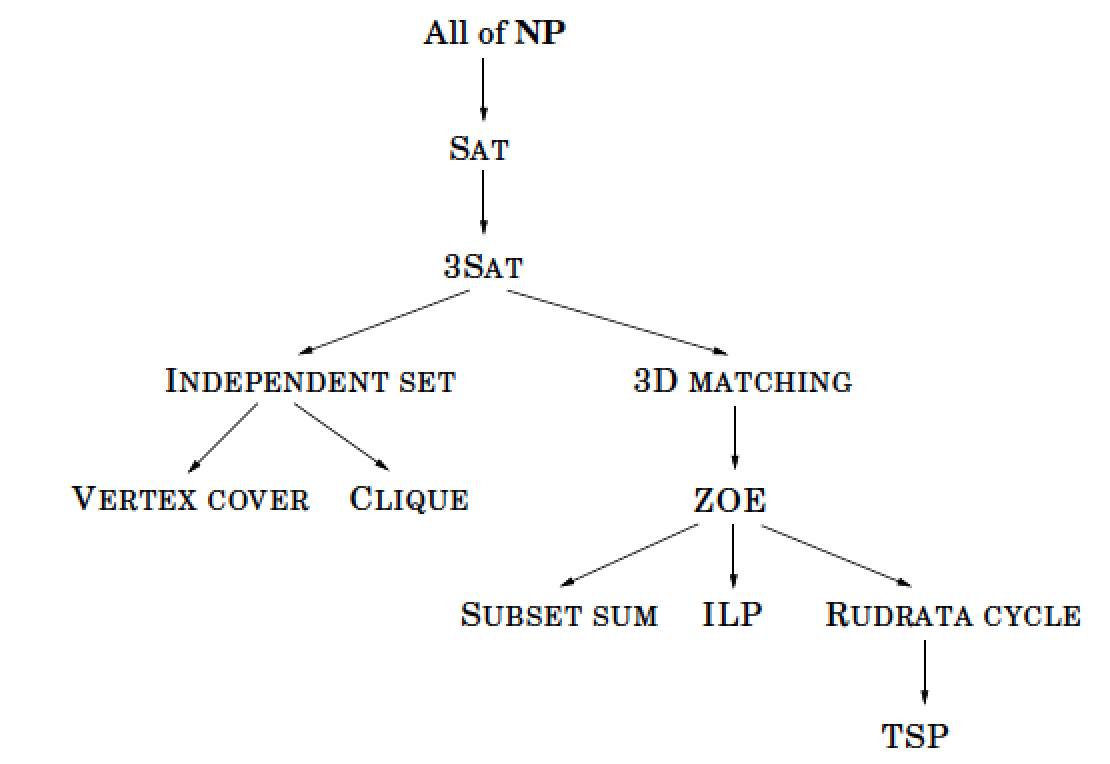
\includegraphics[scale=.4]{Reductions}
\end{center}
% You can even have references
\rule{0.3\linewidth}{0.25pt}
\scriptsize
\bibliographystyle{abstract}
\bibliography{refFile}
\end{multicols}
\end{document}
